\section{Performantie van de Controllers}
\label{sec:performance}
Laten we nu de performantie van onze controllers beschouwen. We kijken hierbij naar de gemiddelde snelheid, topsnelheid, neiging tot driften en hoe robuust de controller is. We geven hierbij ook aan welke circuits de controllers al dan niet kunnen afleggen. In Tabel~\ref{tbl:controllerresultaten} lijsten we de beste resultaten op van de algemene controllers. Bij het produceren van deze resultaten liepen de wagens geen schade op.

\begin{table}
	\centering
	\caption{Beste resultaten van algemene controllers}
	\label{tbl:controllerresultaten}
	
	\begin{subtable}{\linewidth}
   		\centering
   		\caption{Safecontroller}
   		\label{tbl:resultssafe}
       	\begin{tabular}{lrrrr}
        	\toprule
        	Track             & Tijd (s) & Drift (m) & Drift (s) & Top speed 
        	(km/h) \\
        	\midrule
        	Interlagos        & 233.141 & 0 & 0 & 72.06 \\ 
        	Texas             & 121.763 & 0 & 0 & 71.24 \\
        	Spa-Francorchamps &       / & / & / & / \\
        	Silverstone       & 178.367 & 0 & 0 & 71.91 \\
        	\bottomrule
    	\end{tabular}
   	\end{subtable}
   	
	\begin{subtable}{\linewidth}
   		\centering
   		\caption{Speedcontroller}
   		\label{tbl:resultsspeed}
   		\begin{tabular}{lrrrr}
    		\toprule
        	Track             & Tijd (s) & Drift (m) & Drift (s) & Top speed  
        	(km/h) \\
        	\midrule
        	Interlagos        & 128.100 &      0 &     0 & 304.16 \\
        	Texas             &  59.369 & 257.11 & 4.799 & 352.73 \\
        	Spa-Francorchamps &       / &      / &     / &      / \\
        	Silverstone       & 106.700 &   20.5 & 1.600 & 270.97 \\
        	\bottomrule
    	\end{tabular}
   	\end{subtable}
  	   	
   	\begin{subtable}{\linewidth}
   		\centering
   		\caption{Driftcontroller}
   		\label{tbl:resultsdrift}
   	    \begin{tabular}{lrrrr}
   	    \toprule
       	Track             & Tijd (s) & Drift (m) & Drift (s) & Top speed  
       	(km/h) \\
   	    \midrule
       	Interlagos        & 116.081 & 117.29 & 4.342 & 244.47 \\
       	Texas             &  58.034 & 277.37 & 5.000 & 336.69 \\
       	Spa-Francorchamps &       / &      / &     / &      / \\
       	Silverstone       & 109.533 &  66.42 & 2.767 & 272.75 \\
   	    \bottomrule
   	    \end{tabular}
   	\end{subtable}
\end{table}

In de tabel zien we dat er geen gegevens beschikbaar zijn voor het circuit van Spa-Francorchamps. Geen enkele controller was namelijk in staat om door de laatste bocht te raken. Deze bocht is namelijk scherper dan 150 graden (zie Figuur~\ref{fig:spa}) waardoor de zijwaartse scanners niet kunnen uitmaken in welke richting de bocht gaat. Doordat onze controller steeds in de richting rijdt waarheen deze het verste kan kijken zal deze dus beslissen om rechtdoor te gaan, tegen de muur. Hierna zal deze de bocht ook niet meer verlaten.

\begin{figure}[h]
\centering
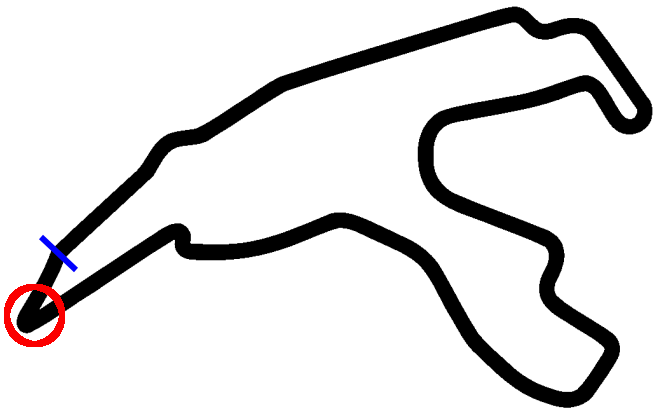
\includegraphics[width=.5\textwidth]{spa_circuit_bocht}
\caption{Circuit van Spa-Francorchamps met de laaste bocht aangeduid met rood}\label{fig:spa}
\end{figure}

De controllers presteren in het algemeen het beste op banen die breed zijn en 
egale bochten hebben, zoals Texas en Interlagos. Op een circuit zoals 
Silverstone en Spa-Francorchamps waar enkele zeer scherpe bochten en scherpe 
slaloms in verwerkt zijn moeten we voorzichtiger rijden met de speedcontroller en durft de driftcontroller al eens uit de bocht te gaan.

\subsection{Veiligheid}

In het geval van de veilige controller zien we dat deze de gemiddelde snelheid 
begrenst wordt tot de bovengrens van \texttt{slow}. Op de rechte stukken 
spreken we hier dus van een topsnelheid van ongeveer 70 km/h. Wanneer deze 
controller bochten tegenkomt zal deze remmen. De snelheid daalt hierbij dan 
daar 50 km/h. Dit trage gedrag zien we duidelijk in Tabel~\ref{tbl:resultssafe} 
aan de rondetijden. Ook zal er bij deze lagere snelheden geen mogelijkheid zijn 
om te driften. 

Verder zal door onze manier van sturen ertoe leiden dat de wagen zelfs op rechte stukken kleine correcties probeert te maken. Dit zou opgevangen moeten worden door het vage regelsysteem maar dit is niet voldoende het geval. Volgens ons is dit te wijten aan \texttt{corner}-invoer. Deze zal namelijk zeer snel aangeven dat er een milde bocht is. Daarnaast zijn de randen van het parcours grillig, wat er nog sneller voor zal zorgen dat de controller beslist om bij te sturen.

Doordat we onze sturing baseren op een locatie die een eind voor de wagen ligt zullen we ook niet naar het midden van de baan sturen maar naar het midden van de baan in de verte. Concreet zal de wagen dus meer naar de binnenkant van de bocht neigen.

De veilige controller blijkt zeer robuust te zijn. De lijn die deze controller doorheen het parcours zal nemen is bijna exact dezelfde doordat de snelheid van de wagen ook steeds dezelfde zal zijn.
\subsection{Snelheid}
De snelle controller is in staat om de circuits van Silverstone en Interlagos af
te leggen zonder te crashen. De snelheid zal hier vari\"eren van 80
km/h in de bochten tot 130 km/h op de rechte stukken. Bij lange rechte stukken
is het mogelijk dat de wagen hogere snelheden behaalt, de topsnelheid die wij op
deze circuits waargenomen hebben is $304.16$ km/h.

Op het snelle circuit van Texas zal de controller zeer hoge snelheden behalen
maar niet op tijd beginnen remmen. De controller zal dus tegen een hoge snelheid
de bocht proberen nemen en bijgevolg slippen en crashen of een lus maken. Ondanks de crash zal
deze controller zeer snelle tijd neerzetten op het circuit. De topsnelheid die we hier meten is $352.73$ km/h.

Zoals we in Tabel~\ref{tbl:resultsspeed} kunnen zien zal de snelle controller ook aanleg hebben tot driften maar zal hier niet op doelen. Zo zien we dat deze op het circuit van Interlagos zijn snelste ronde neerzet zonder te driften. Ook op Silverstone blijft de drift beperkt. Door de crash in Texas zal hier natuurlijk een hoge driftscore verschijnen.

De robuustheid van deze controller ligt al een stuk lager dan die van de veilige controller. Wanneer de wagen namelijk uit een bocht komt en een lang recht stuk nadert, zal de wagen enkel sterk versnellen indien de wagen op tijd stabiel genoeg is. Indien de wagen maar net stabiel genoeg is zal de wagen mogelijks toch versnellen en dus heen en weer schommelen op het rechte stuk met een crash tot gevolg. De snelle controller zal dus ongeveer één op de tien keer crashen op de circuits van Silverstone en Interlagos.
\subsection{Drift}
Omdat de driftcontroller gebaseerd is op de snelle controller zien we 
gelijkaardige resultaten. Door te driften zien we echter voor Interlagos een 
betere tijd opduiken.

Zoals besproken bij de implementatie van deze controller is deze controller een 
gewaagde versie van de speedcontroller waarbij we meer risico's nemen zoals 
later remmen, oversturen, meer gas geven bij het verlaten van de bocht, etc. 
Daarom zien we ook dat deze controller meer crasht dan de speedcontroller. 

Het parcour op Interlagos is perfect voor deze controller. Door de wijde 
bochten waarvan de hoek de hele bocht gelijk blijft drift hij zich hier vaak 
mooi door. Omdat we sneller door de bochten durven gaan de speedcontroller, 
alsook op de rechte stukken goed gas durven geven halen we hier zelfs een 
snellere tijd dan bij de speedcontroller, al ligt de topsnelheid een stuk 
lager. Bij de lange stukken durft hij wel eens de controle over het stuur 
te verliezen door kleine stuurcorrecties, of niet genoeg afremmen bij het 
insturen van een bocht. Ditzelfde gedrag zien we ook vaak bij Texas de kop 
opsteken.

Als we naar de tabel kijken in Tabel~\ref{tbl:resultsdrift} zien we dat de 
wagen ook effectief meer drift dan de andere controllers.

Op het parcours van Silverstone en Spa-Francorchamps presteert deze controller 
veel minder goed en mogen we al blij zijn dat hij (in het geval van 
Silverstone) het parcours uitrijdt. De wagen probeert zich vaak door bochten te 
driften, maar aangezien die vaak te scherp zijn heeft hij hier meestal de 
snelheid niet voor.

De robuustheid van deze controller ligt nog lager dan die van die van de 
speedcontroller. Rechte stukken worden soms snel genomen, soms niet. De ene 
keer drift hij goed door bochten, waar hij de volgende keer traag zonder 
driften door rijdt. De oorzaak hiervan is dat het gedrag een stuk minder 
gecontroleerd en een stuk meer bruusk is dan bij andere controllers.
